\documentclass[sigconf,natbib=true,anonymous]{acmart}
%% WSDM 2027 Main Track draft (9 pages + unlimited references + ethics)
%% Double-blind review. Camera-ready: remove 'anonymous' and add authors.

\settopmatter{printacmref=false}
\renewcommand\footnotetextcopyrightpermission[1]{}
\setcopyright{none}
\acmConference[WSDM'27]{Proceedings of the 20th ACM International Conference on Web Search and Data Mining}{February 15--19, 2027}{Hong Kong}
\acmYear{2027}
\acmDOI{}
\acmISBN{}

\usepackage{booktabs}
\usepackage{multirow}
\usepackage{amsmath,amssymb}
\usepackage{graphicx}
\usepackage{subcaption}
\usepackage{siunitx}
\usepackage{xspace}
\usepackage{enumitem}
\usepackage{microtype}
\usepackage{balance}
\usepackage{hyperref}

\newcommand{\tfidf}{\textsc{TF-IDF}\xspace}
\newcommand{\llm}{\textsc{LLM}\xspace}
\newcommand{\base}{\textsc{SASRec}\xspace}

\begin{document}

\title{When More Text Is Not Better:\\
A Leakage-Aware Study of Text Representations\\
for Sequential Recommendation}

\author{Anonymous Author(s)}
\affiliation{%
  \institution{Anonymous Institution}
  \country{}}
\renewcommand{\shortauthors}{Anonymous}

\begin{abstract}
Text features are widely used to enhance sequential recommenders, yet most evidence comes from leave-one-out (LOO) protocols that allow training and test interactions to overlap in time.
We conduct a leakage-aware controlled study of four text representations---ID-only, lexical \tfidf, single-view large language model (\llm) embeddings, and prompt-based multi-view \llm features---under global temporal split (GTS) and clean LOO on Amazon Beauty and Toys.
Three findings emerge.
First, the protocol changes conclusions: under GTS, \tfidf is strongest (Beauty MRR@10 $0.0165$; Toys $0.0113$), whereas under LOO, single-view \llm and multi-view become competitive or slightly better, with absolute metrics substantially inflated.
Second, across Main and Early temporal windows, \tfidf remains the most stable, while \llm/multi-view do not exceed it by one standard deviation.
Third, multi-view does not yield reliable gains: pairwise CKA among four prompt views is $0.82$--$0.94$, concatenating views collapses effective rank to $\approx$53\% of dimensionality, and leave-one-view-out changes MRR by at most $0.03$ percentage points.
In contrast, CKA between \tfidf and \llm views is only $\approx$0.19--0.20, suggesting lexical and semantic features are complementary rather than redundant.
Together, these results argue that strict temporal evaluation can reverse rankings among text representations, and that more semantic views do not automatically provide more useful information.
\end{abstract}

\begin{CCSXML}
<ccs2012>
 <concept>
  <concept_id>10002951.10003317.10003347.10003350</concept_id>
  <concept_desc>Information systems~Recommender systems</concept_desc>
  <concept_significance>500</concept_significance>
 </concept>
 <concept>
  <concept_id>10002951.10003317.10003318.10003319</concept_id>
  <concept_desc>Information systems~Content ranking</concept_desc>
  <concept_significance>300</concept_significance>
 </concept>
</ccs2012>
\end{CCSXML}
\ccsdesc[500]{Information systems~Recommender systems}
\ccsdesc[300]{Information systems~Content ranking}

\keywords{Sequential Recommendation, Text Features, Temporal Evaluation, Multi-View Representation, Leakage-Aware Protocol}

\maketitle

%==============================================================================
\section{Introduction}
%==============================================================================

Sequential recommendation predicts a user's next item from historical interactions~\cite{kang2018sasrec,sun2019bert4rec,hidasi2016gru4rec}.
Item text---titles, descriptions, and LLM-encoded semantics---has become a standard way to enrich ID embeddings~\cite{hou2022unisrec,hou2023vqrec,bao2023tallrec}.
A common intuition is that richer text should help: \llm embeddings should beat bag-of-words, and multiple prompt views should beat a single view.

This intuition is fragile under realistic evaluation.
Most text-enhanced sequential recommenders are still validated with leave-one-out (LOO) splits, which can leak future interactions into training and inflate absolute metrics~\cite{ji2023evaluation,sun2023reevaluation}.
Global temporal split (GTS) enforces a train/valid/test cutoff and better matches deployment, but it also exposes distribution shift: catalog turnover, cold targets, and popularity decay.
Prior work has studied split choices in general~\cite{meng2020temporal,krichene2020sampledmetrics}; our focus is narrower and more actionable for practitioners who choose among \emph{text representations}:
does the protocol change the ranking of \tfidf vs.\ single-view \llm vs.\ prompt multi-view?

We study this question with a controlled, leakage-aware protocol.
All text features (vocabulary/\tfidf, SVD, centering/whitening, LLM embeddings) are fit only on items observed before the training cutoff.
We compare five systems on Amazon Beauty and Toys under clean LOO and GTS, with a frozen Early temporal window and UniSRec~\cite{hou2022unisrec} as an external text baseline.
We further diagnose multi-view failure with CKA~\cite{kornblith2019cka}, effective rank, and leave-one-view-out (LOOV).

\noindent\textbf{Research questions.}
\begin{enumerate}[leftmargin=*,itemsep=1pt]
\item[\textbf{RQ1}] Does switching from LOO to GTS change conclusions about \tfidf, single-view \llm, and multi-view text?
\item[\textbf{RQ2}] Which text representation is most robust across temporal windows under distribution shift?
\item[\textbf{RQ3}] Why does prompt-based multi-view fail to reliably beat single-view?
\end{enumerate}

\noindent\textbf{Contributions.}
(1)~A leakage-aware comparison showing that GTS reverses LOO rankings among text representations.
(2)~Evidence that \tfidf is the most stable under Main/Early windows, associated with (not claimed as caused by) rising unseen-target share and catalog turnover.
(3)~Triangulated redundancy analysis (CKA + effective rank + LOOV) explaining why more prompt views do not help, while lexical \tfidf remains complementary to semantic \llm features.

%==============================================================================
\section{Related Work}
%==============================================================================

\paragraph{Text-enhanced sequential recommendation.}
Early work fused bag-of-words or review text with collaborative filtering~\cite{wang2015cdl,salton1988termweighting}.
Recent systems encode titles/descriptions with pretrained language models and transfer them across domains~\cite{hou2022unisrec,hou2023vqrec,geng2022p5,bao2023tallrec}.
We deliberately do \emph{not} propose a new architecture; instead we ask whether stronger text encoders and more views remain advantageous once temporal leakage is controlled.

\paragraph{Evaluation protocols and temporal leakage.}
Sampled metrics can distort rankings~\cite{krichene2020sampledmetrics}.
LOO vs.\ time-based splits systematically change absolute scores and can alter model selection~\cite{ji2023evaluation,sun2023reevaluation,meng2020temporal}.
We follow this line but specialize it to text representations: protocol effects matter precisely because \tfidf, \llm, and multi-view respond differently to temporal shift.

\paragraph{Multi-view learning.}
Multi-view theory emphasizes \emph{useful complementary} information rather than ``more views''~\cite{xu2013multiview}.
Representation similarity tools such as CKA~\cite{kornblith2019cka} help detect redundancy.
Our prompt views share the same encoder and item title, making redundancy a first-order risk.

%==============================================================================
\section{Leakage-Aware Protocol and Models}
%==============================================================================

\subsection{Temporal Protocols}
\label{sec:protocol}

\paragraph{Global Temporal Split (GTS).}
Interactions are ordered by timestamp.
We use RecBole's \texttt{TS} split~\cite{zhao2021recbole} with ratios $[0.8,0.1,0.1]$ (Main) or $[0.6,0.1,0.3]$ (Early).
A global cutoff places the final 10\% (Main) of interactions into test; train/valid are further split within the pre-test window.
After sequential augmentation, \emph{all} post-cutoff next-item steps enter evaluation (\textbf{GTS-All}).
This matches how RecBole SequentialDataset evaluates successive targets after a time cutoff.
Appendix~\ref{app:gts-last} reports a GTS-Last re-evaluation (one last target per user) on the same checkpoints.

\paragraph{Clean LOO.}
For contrast, we also run leave-one-out evaluation without temporal cutoff (train/valid/test as last-3 interactions per user), using the same model family and hyperparameters.
LOO is \emph{not} used for main conclusions.

\paragraph{Leakage controls.}
\tfidf vocabulary/IDF, SVD projection, and LLM center/whitening are fit \textbf{only} on items appearing before the training cutoff.
Evaluation optionally restricts to users with $\ge 5$ training interactions (\texttt{min\_train\_interactions=5}).
Warm-target analyses keep only targets present in the train catalog; unseen targets are reported separately (Appendix).

\subsection{Model Variants}
All models share a \base~\cite{kang2018sasrec} backbone ($d{=}64$, 2 blocks) unless noted.
\begin{itemize}[leftmargin=*,itemsep=1pt]
\item \textbf{ID}: ID embeddings only.
\item \textbf{TF}: train-cutoff \tfidf (SVD to 256-d) fused via a lightweight text head + InfoNCE alignment~\cite{oord2018cpc}.
\item \textbf{LLM}: single-view Qwen2.5-7B~\cite{qwen2024qwen25} item embedding (TS-whitened), same fusion.
\item \textbf{MV}: four prompt views (Description / Function / Audience / Style), concatenated then projected; no cross-attention in the main table.
\item \textbf{UniSRec}: external text sequential baseline~\cite{hou2022unisrec} with the same TS embeddings and GTS filter for fair comparison.
\end{itemize}
Two-phase training (text-head warmup, then joint fine-tuning) is used for TF/LLM/MV.
Cross-attention variants are relegated to Appendix as negative results.

%==============================================================================
\section{Experimental Setup}
%==============================================================================

\paragraph{Datasets.}
Amazon Beauty and Toys \& Games~\cite{mcauley2015amazon,ni2019amazon}.
Beauty: 1.21M users, 259K items, 2.02M interactions.
Toys: larger catalog (336K items) with similar sparsity.

\paragraph{Metrics.}
Full-ranking Hit@10, NDCG@10, MRR@10~\cite{krichene2020sampledmetrics}.
Main tables report MRR@10 (mean$\pm$std over seeds $\{42,2024,2026\}$).

\paragraph{Compute.}
All runs use RecBole~\cite{zhao2021recbole} with identical full-sort evaluation.
Hyperparameters for Early are frozen from Main (no re-tuning).

%==============================================================================
\section{Results}
%==============================================================================

\subsection{RQ1: Protocol Changes Rankings}
\label{sec:rq1}

\begin{table}[t]
\centering
\caption{Protocol contrast (MRR@10, 3-seed mean$\pm$std, \texttt{min\_train}=5).
\textbf{Bold}: best in row within protocol.
GTS ranking favors \tfidf; LOO favors LLM/MV with inflated absolutes.}
\label{tab:protocol}
\small
\setlength{\tabcolsep}{3.5pt}
\begin{tabular}{@{}llcccc@{}}
\toprule
Dataset & Protocol & ID & TF-IDF & LLM & MV \\
\midrule
\multirow{2}{*}{Beauty}
 & GTS & $.0106{\scriptstyle\pm.0005}$ & $\mathbf{.0165{\scriptstyle\pm.0008}}$ & $.0161{\scriptstyle\pm.0005}$ & $.0160{\scriptstyle\pm.0008}$ \\
 & LOO & $.0175{\scriptstyle\pm.0004}$ & $.0251{\scriptstyle\pm.0002}$ & $\mathbf{.0254{\scriptstyle\pm.0004}}$ & $.0253{\scriptstyle\pm.0004}$ \\
\midrule
\multirow{2}{*}{Toys}
 & GTS & $.0070{\scriptstyle\pm.0001}$ & $\mathbf{.0113{\scriptstyle\pm.0003}}$ & $.0107{\scriptstyle\pm.0004}$ & $.0109{\scriptstyle\pm.0006}$ \\
 & LOO & $.0152{\scriptstyle\pm.0005}$ & $.0247{\scriptstyle\pm.0006}$ & $\mathbf{.0258{\scriptstyle\pm.0012}}$ & $\mathbf{.0258{\scriptstyle\pm.0028}}$ \\
\bottomrule
\end{tabular}
\end{table}

\begin{figure}[t]
\centering
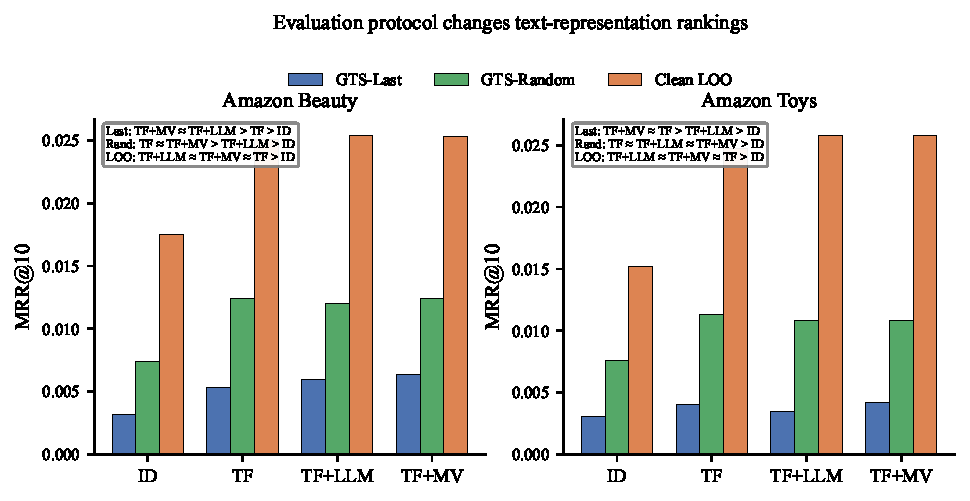
\includegraphics[width=\linewidth]{figures/fig_protocol_contrast.pdf}
\caption{LOO vs.\ GTS on Beauty and Toys.
Bars are 3-seed mean MRR@10.
Ranking annotations highlight the protocol-induced flip.}
\label{fig:protocol}
\end{figure}

Table~\ref{tab:protocol} and Figure~\ref{fig:protocol} answer RQ1.
Under GTS, text still beats ID by a large margin, but \textbf{\tfidf $\ge$ LLM $\approx$ MV}.
Under clean LOO, absolute MRR rises by $\sim$1.5--2$\times$, and the ranking becomes \textbf{LLM $\approx$ MV $\ge$ TF}.
Thus the protocol does not merely rescale scores---it changes which text representation looks best.
This is consistent with prior temporal-evaluation warnings~\cite{ji2023evaluation,sun2023reevaluation}, specialized here to TF/LLM/MV.

\paragraph{External baseline.}
With the same GTS + \texttt{min\_train}=5 filter, UniSRec scores $0.0123{\scriptstyle\pm.0001}$ (Beauty) and $0.0082{\scriptstyle\pm.0001}$ (Toys)---\emph{below} our TF/LLM align models.
Earlier UniSRec ``wins'' disappeared once the eval filter was equalized.

\subsection{RQ2: Temporal Robustness}
\label{sec:rq2}

\begin{table}[t]
\centering
\caption{Main vs.\ Early temporal window on Beauty (MRR@10 test, 3 seeds).
Hyperparameters frozen from Main.
Early: \texttt{TS}$[0.6,0.1,0.3]$.}
\label{tab:early}
\small
\begin{tabular}{@{}lccc@{}}
\toprule
Window & TF-IDF & LLM & MV \\
\midrule
Main (GTS) & $\mathbf{.0165{\scriptstyle\pm.0008}}$ & $.0161{\scriptstyle\pm.0005}$ & $.0160{\scriptstyle\pm.0008}$ \\
Early60 & $\mathbf{.0053{\scriptstyle\pm.0002}}$ & $.0049{\scriptstyle\pm.0002}$ & $.0052{\scriptstyle\pm.0001}$ \\
\bottomrule
\end{tabular}
\end{table}

\begin{table}[t]
\centering
\caption{Temporal distribution shift (valid$\rightarrow$test under Main GTS).
We report \emph{associations}, not causal claims.}
\label{tab:shift}
\small
\setlength{\tabcolsep}{4pt}
\begin{tabular}{@{}lcccc@{}}
\toprule
Dataset & Test new-item & Test unseen bucket & Pop mean (V$\rightarrow$T) & Pop p50 (V$\rightarrow$T) \\
\midrule
Beauty & 27.3\% & 17.8\% & $112.8\rightarrow101.8$ & $21\rightarrow15$ \\
Toys & 32.8\% & 21.3\% & $144.7\rightarrow119.1$ & $18\rightarrow11$ \\
\bottomrule
\end{tabular}
\end{table}

Table~\ref{tab:early} shows that Early window preserves the Main ordering: \tfidf remains strongest; LLM/MV never exceed it by one std.
Absolute scores drop sharply (Main$\rightarrow$Early), concurrent with the distribution statistics in Table~\ref{tab:shift}: higher catalog novelty, more unseen targets, and lower target popularity from valid to test.
Warm-target audit (eligible users, hist$\ge$5) similarly finds test unseen shares of 27.8\% (Beauty) and 34.5\% (Toys).
We phrase these as associations with the valid$\rightarrow$test performance drop (43--55\% in our runs), not as proven causes.

\subsection{RQ3: Why Multi-View Does Not Help}
\label{sec:rq3}

\begin{figure}[t]
\centering
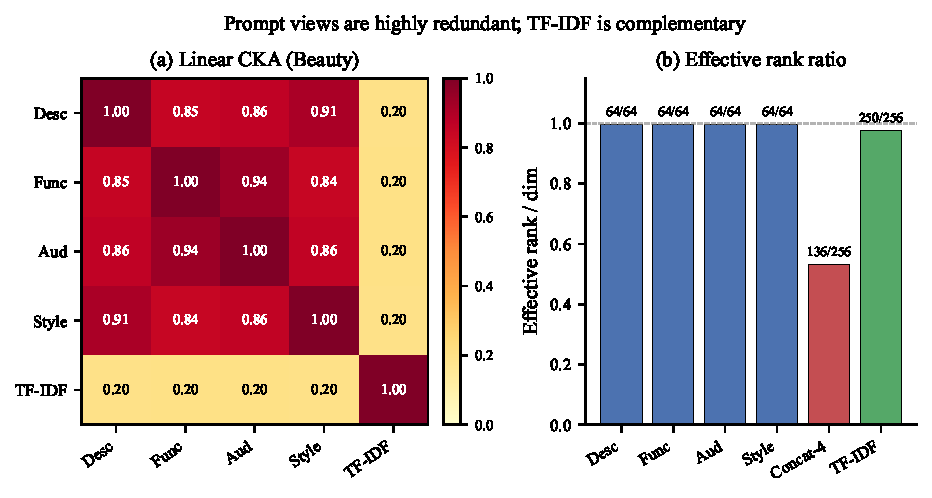
\includegraphics[width=\linewidth]{figures/fig_cka_heatmap.pdf}
\caption{Representation analysis on Beauty (3 item subsamples of 3{,}000).
(a)~Inter-view CKA is high ($0.84$--$0.94$); TF--LLM CKA is low ($\approx0.20$).
(b)~Concatenating four 64-d views yields effective rank $136/256$ (ratio $0.53$), vs.\ TF-IDF $250/256$ ($0.98$).}
\label{fig:cka}
\end{figure}

\begin{table}[t]
\centering
\caption{Leave-one-view-out (zero-mask) on GTS MV checkpoints (seed~42).
$\Delta$ is MRR@10 change vs.\ full 4-view model.}
\label{tab:loov}
\small
\setlength{\tabcolsep}{3pt}
\begin{tabular}{@{}llrrrr@{}}
\toprule
Dataset & Full & $-\,$Desc & $-\,$Func & $-\,$Aud & $-\,$Style \\
\midrule
Beauty & .01591 & $-$.00006 & $+$.00011 & $-$.00016 & $-$.00034 \\
Toys & .01018 & $-$.00019 & $-$.00011 & $-$.00012 & $-$.00015 \\
\bottomrule
\end{tabular}
\end{table}

\begin{table}[t]
\centering
\caption{Parameter count and inference cost (seed~42, Beauty).
MV adds $<$1\% parameters and negligible latency.}
\label{tab:cost}
\small
\begin{tabular}{@{}lcc@{}}
\toprule
Model & Params (M) & ms / sample \\
\midrule
ID / TF / LLM / MV & 67.16 / 67.43 / 67.56 / 67.71 & 0.02 \\
UniSRec & 67.69 & 0.04 \\
\bottomrule
\end{tabular}
\end{table}

Figure~\ref{fig:cka} and Table~\ref{tab:loov} address RQ3.
Four prompt views are structurally redundant: inter-view CKA ranges $0.82$--$0.94$ (Toys similar), while concat effective-rank ratio is only $0.53$ (Beauty) / $0.55$ (Toys).
LOOV deltas are tiny ($|\Delta|{<}0.0004$), i.e., $<$3\% relative to full MV MRR.
CKA alone does not prove uselessness~\cite{kornblith2019cka}, but CKA + effective rank + LOOV together support the claim that prompt views largely restate the same semantics.
Meanwhile TF--LLM CKA $\approx0.19$--$0.20$ indicates lexical and semantic features are complementary---yet simply stacking four \llm prompts does not harvest that complementarity.
Table~\ref{tab:cost} shows the failure is not due to capacity: MV has essentially the same parameter/latency budget as TF/LLM.

\subsection{Takeaways for Practitioners}
\begin{enumerate}[leftmargin=*,itemsep=2pt]
\item Prefer GTS (or another leakage-controlled temporal protocol) when comparing text representations; LOO can reverse rankings and inflate scores.
\item Start with cutoff-fit \tfidf before investing in multi-prompt \llm views.
\item If using \llm text, a single view often matches four; diagnose redundancy before scaling views.
\end{enumerate}

%==============================================================================
\section{Conclusion}
%==============================================================================

We reframed text-enhanced sequential recommendation as a leakage-aware empirical study rather than a race for a new SOTA model.
Under GTS, \tfidf is competitive or best; under LOO, \llm/multi-view look stronger.
Temporal windows and distribution-shift statistics reinforce that semantic multi-view gains are not robust, and representation analyses explain why: prompt views are redundant, while lexical and semantic features are complementary but not exploited by naive multi-prompt stacking.
Future work includes GTS-Last/Random as primary tables, successive evaluation at scale, and hybrid TF+\llm fusion that targets complementarity rather than view count.

\section*{Ethical Considerations}
This work uses public Amazon review datasets without personally identifiable private attributes beyond standard user/item IDs.
Potential harms include reinforcing popularity bias under temporal shift and over-trusting LLM text features that may encode stereotypes present in product descriptions.
We mitigate the first by reporting stratified/warm-target diagnostics; the second by treating multi-view LLM features as an empirical object of study rather than a default upgrade.
No human subjects were involved.

\begin{acks}
Anonymous for review.
\end{acks}

\bibliographystyle{ACM-Reference-Format}
\bibliography{refs}

%==============================================================================
\appendix
\section{GTS-Last Re-evaluation}
\label{app:gts-last}
%==============================================================================

Our main GTS tables use Successive-All targets (Beauty: 4{,}520 users $\rightarrow$ 12{,}001 test samples).
Re-evaluating the same checkpoints with \textbf{GTS-Last} (one last target per user) yields lower absolute MRR and a milder ranking change (Beauty mean MRR@10: ID $0.0022$, TF $0.0036$, LLM $0.0041$, MV $0.0042$; Toys: ID $0.0019$, TF $0.0025$, LLM $0.0022$, MV $0.0026$).
This confirms that target selection is part of the protocol definition and should be stated explicitly; we keep GTS-All as the RecBole-native main setting and report Last for completeness.

\section{Warm-Only Targets}
\label{app:warm}
%==============================================================================

Restricting GTS test targets to the train catalog raises absolute MRR but preserves GTS ranking (Beauty warm MRR: TF $0.0242$, LLM/MV $0.0236$; Toys: TF $0.0191$, LLM $0.0181$, MV $0.0184$).
Unseen-item shares under this filter are 31.9\% (Beauty) and 40.8\% (Toys).

\section{Cross-Attention (Negative Result)}
\label{app:cross}
%==============================================================================

Optional sequence--text cross attention improves and degrades roughly equally across users; score entropy/margin shifts are unstable across seeds.
We therefore exclude Cross from the main method and title, retaining it only as a negative appendix observation.

\end{document}
